\documentclass[a4paper,norsk]{article}
\usepackage[latin1]{inputenc}
\usepackage[T1]{fontenc}
\usepackage{babel,textcomp,listings, subfigure,graphicx}
\usepackage{subfig}
\usepackage{amsmath}
                                    
\title{Assignment 2, Mek4250}
\author{Sebastian Gjertsen}
\begin{document}
\maketitle
\section*{1}
\subsection*{7.1}
First we have to show:
$$ a(u,v) \leq C ||u||_{H^1_0} ||v||_{H^1_0}  $$
We start with:
\begin{align*}
\int \nabla u : \nabla v dx &\leq (\int (\nabla u  \nabla v)^2 dx)^{\frac{1}{2}} = \\
& \text{Using Cauchy- Schwartz} \\
||\nabla u \nabla v||_{L^2} & \leq  C ||\nabla u||_{L^2} ||\nabla v||_{L^2} = \\
C|u|_{H^1_0} |v|_{H^1_0} & \leq C ||u||_{H^1_0} ||v||_{H^1_0}\\
\end{align*}
The last line we can see is true since the H1 seminorm has to be smaller than the H1 norm since it contains the L2 norm of u in addition to the gradient of u. \newline
Next we want to show:
$$ b(q,u)  \leq C||u||_{H^1_0} ||q||_{L^2}  $$
\begin{align*}
\int q \nabla * u dx &\leq (\int (q \nabla * u)^2 dx)^{\frac{1}{2}} \leq ||q||_{L^2} ||\nabla * u||_{L^2} \text{used Cauchy Schwartz}\\ 
	&\text{Since we now have sorted the q we can focus on the divergence }\\
	||\nabla * u||_{L^2} &\leq  ||\nabla * u||_{L^2} + ||\frac{\partial u_y}{\partial x} +\frac{\partial u_x}{\partial y}||_{L^2} = ||\nabla u||_{L^2} \leq C ||u||_{H^1} \\
	&\text{we use the same trick as before  and get} \\
	\int q \nabla * u dx & \leq C||u||_{H^1_0} ||q||_{L^2} \\
\end{align*}

Lastly we show:

$$ a(u,u) \geq ||u||^2_{H^1_0}  $$
\begin{align*}
||u||^2_{H^1_0} &= ||u||^2_{L^2} ||\nabla u||^2_{L^2}\\   
	  &\text{using Poincares inequality}
           & \leq D||\nabla u||^2_{L^2} + ||\nabla u||^2_{L^2} = ||\nabla u||^2_{L^2} (D+1) \\
           & = C ||\nabla u||^2_{L^2} \\
           & \leq \int \nabla u : \nabla u dx
\end{align*}



\subsection*{7.6}
$$||u-u_h||_1 + ||p-p_h||_0 \leq C h^\alpha||u|| +  C h^\beta ||p||_{\beta+1}    $$
In the 4 figures we see log log plots of u from the different mixes of function spaces. We seem to get good convergence rates for all the combinations but best when the spaces are only one degree apart. \newline
\begin{tabular}{l*{6}{c}r}
Elements         & $\alpha_u$ & $\alpha_p$   \\
\hline
P4-P3           & 4.23752218115  & 4.07080574134\\
P4-P2           & 2.88750262912  & 2.91633169585 \\
P3-P2           & 2.85257225007  & 2.91774992053\\
P3-P1           & 2.08150448230   & 2.15170883599\\
\end{tabular}
\begin{figure}[h] 
  \label{ fig7} 
  \begin{minipage}[b]{0.5\linewidth}
    \centering
    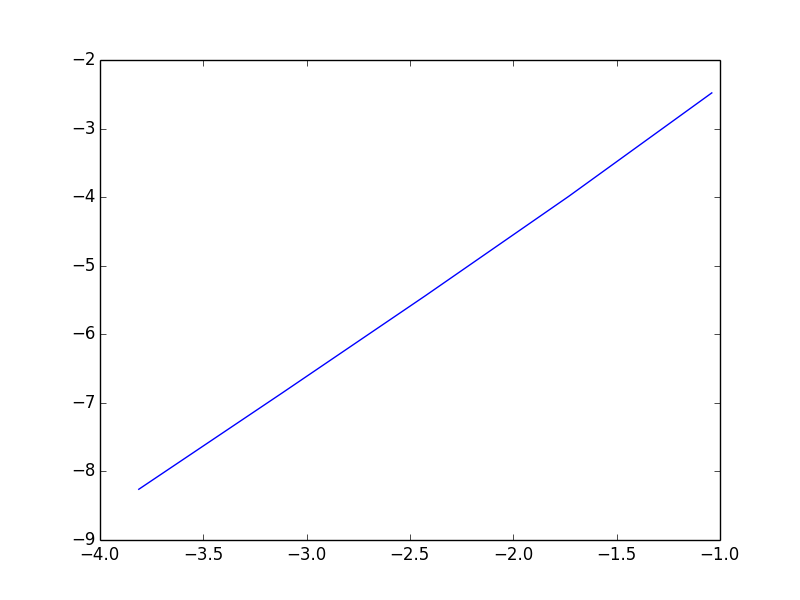
\includegraphics[scale=0.3]{log_plot_p3_p1.png}   
    \caption{P3-P1} 
    \vspace{4ex}
  \end{minipage}%%
  \begin{minipage}[b]{0.5\linewidth}
    \centering
   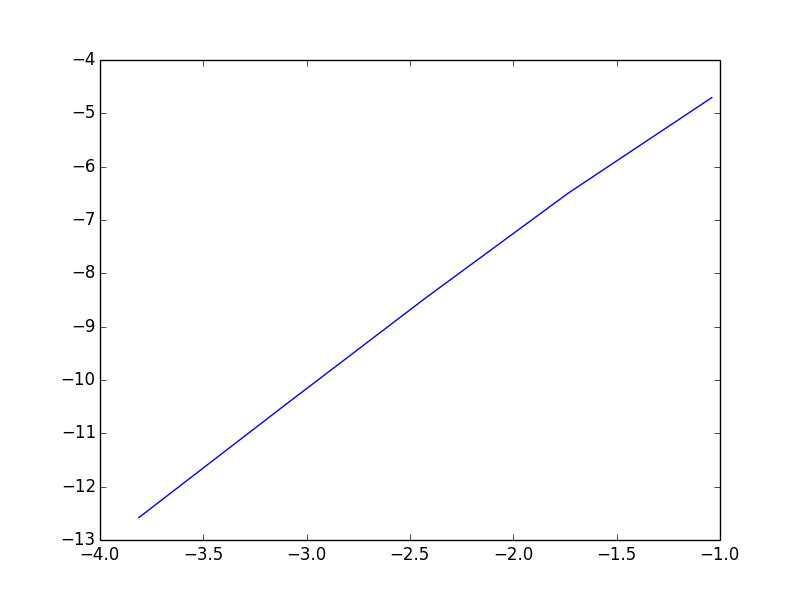
\includegraphics[scale=0.3]{log_plot_p3_p2.png}    
    \caption{P3-P2} 
    \vspace{4ex}
  \end{minipage} 
  \begin{minipage}[b]{0.5\linewidth}
    \centering
    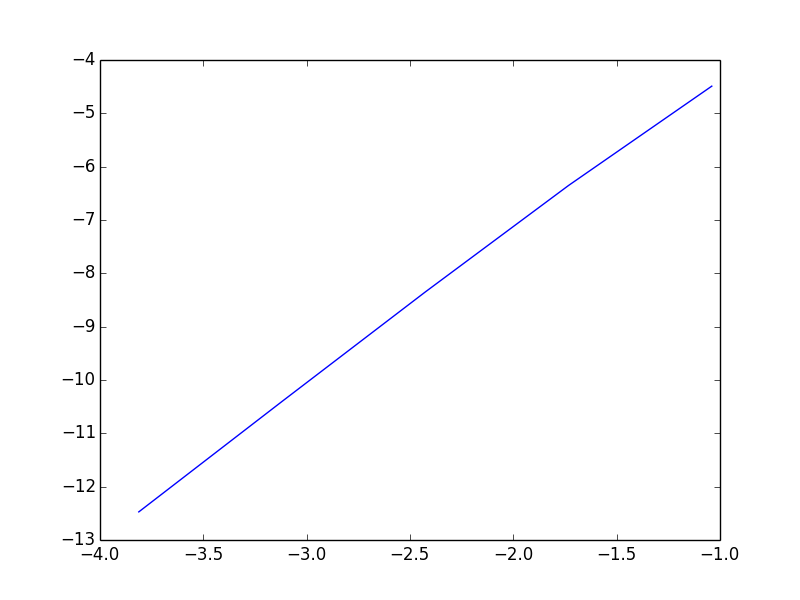
\includegraphics[scale=0.3]{log_plot_p4_p2.png}    
    \caption{P4-P2} 
    \vspace{4ex}
  \end{minipage}%% 
  \begin{minipage}[b]{0.5\linewidth}
    \centering
    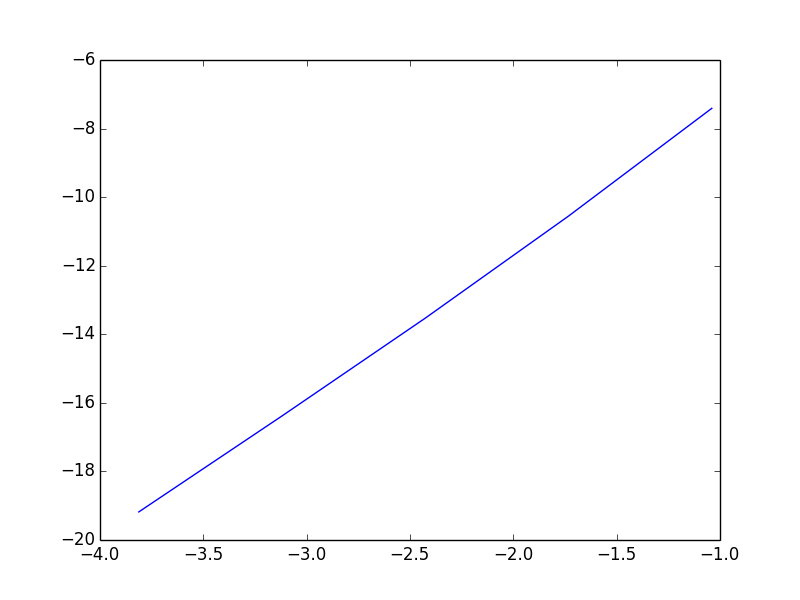
\includegraphics[scale=0.3]{log_plot_p4_p3.png}    
    \caption{P4-P3, } 
    \vspace{4ex}
  \end{minipage} 
\end{figure}
\newpage

\subsection*{7.7}
To calculate the wall shear stress i calculated $\epsilon =  0.5*(\nabla u + \nabla u^T)$, i focused the wall shear stress on the bottom wall and calculated it by hand and got $\epsilon = 0.5*(\pi-2) \approx 0.57$. The convergence was calculated in a similar fashion as 7.6. \newline
\begin{tabular}{l*{6}{c}r}
Elements         & $\alpha_{stress}$   \\
\hline
P4-P3        &  4.08979685189  \\
P4-P2        &  3.47692041535  \\ 
P3-P2        &  2.5719146479 \\
P3-P1        &  3.01745034613 \\
\end{tabular}
\newline

\begin{figure}[h] 
  \label{ fig7} 
  \begin{minipage}[b]{0.6\linewidth}
    \centering
    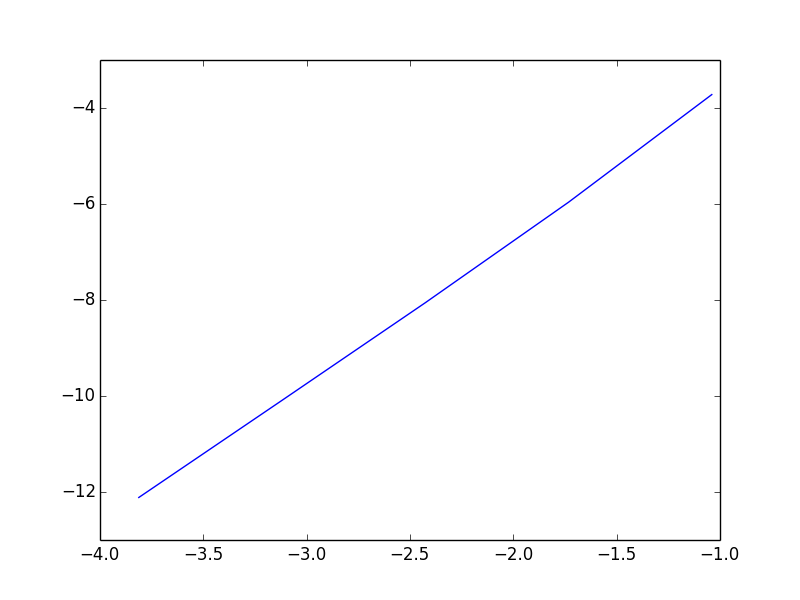
\includegraphics[scale=0.3]{wall_shear_log_plot_p3_p1.png}   
    \caption{P3-P1} 
    \vspace{4ex}
  \end{minipage}%%
  \begin{minipage}[b]{0.6\linewidth}
    \centering
   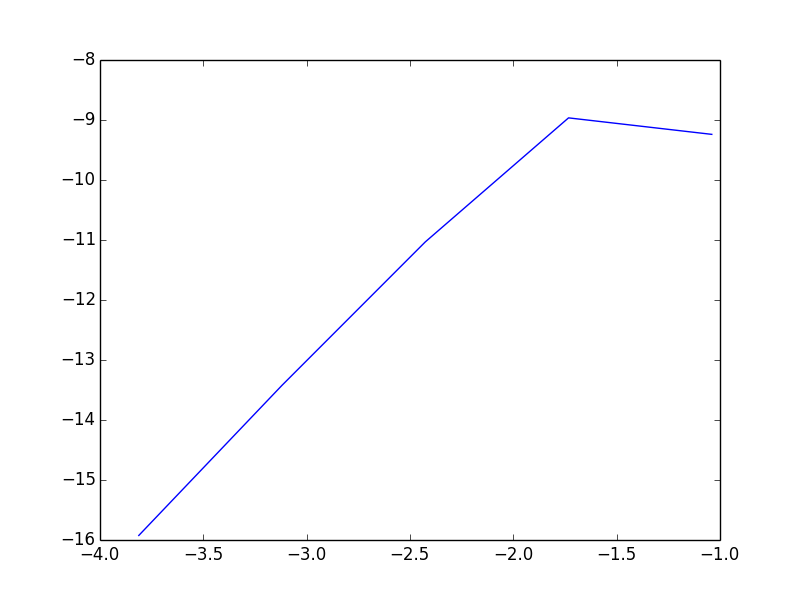
\includegraphics[scale=0.3]{wall_shear_log_plot_p3_p2.png}    
    \caption{P3-P2} 
    \vspace{4ex}
  \end{minipage} 
  \begin{minipage}[b]{0.6\linewidth}
    \centering
    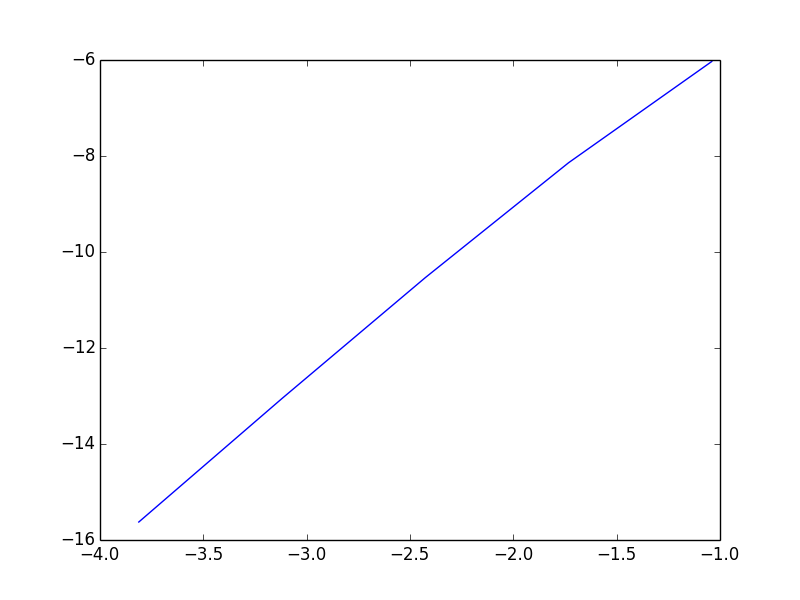
\includegraphics[scale=0.3]{wall_shear_log_plot_p4_p2.png}    
    \caption{P4-P2} 
    \vspace{4ex}
  \end{minipage}%% 
  \begin{minipage}[b]{0.6\linewidth}
    \centering
    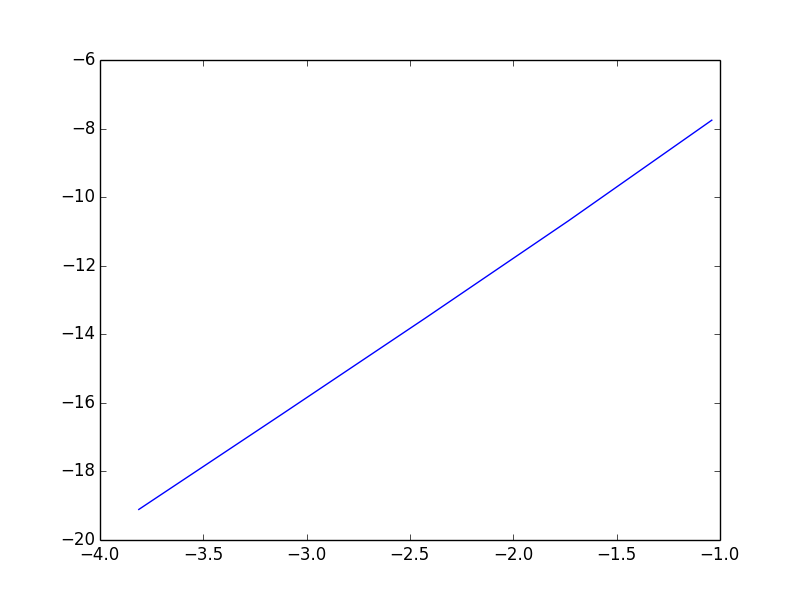
\includegraphics[scale=0.3]{wall_shear_log_plot_p4_p3.png}    
    \caption{P4-P3, } 
    \vspace{4ex}
  \end{minipage} 
\end{figure}



\newpage
\section*{2}
\subsection*{a)}
$$-\mu \nabla u -  \lambda \nabla \nabla * u  = f $$
$$ u_e = (\pi x \cos(\pi x y),-\pi y cos(\pi x y)) $$
I used sympy to calculate the laplacian  of $u_e$ since the divergence term is zero by construction. Giving

$$ f = \big(\pi^2(\pi*x*(x^2+y^2)*cos(\pi x y) + 2 y sin(\pi x y))  ,  \pi^2(\pi*y*(x^2+y^2)*cos(\pi x y) + 2 y sin(\pi x y))       \big) $$


\lstinputlisting[language=Python]{test.py}

\subsection*{b)}
The equation was solved on the form:
$$   \nu(\nabla u, \nabla v) - \lambda (\nabla \nabla *u,v) = (f,v)    $$

\begin{tabular}{l*{6}{c}r}
 & & Errornorm for u  P1 &  \\
\hline
N / $\lambda$      &1 & 100 & 1000  \\
\hline
8   &   6.917632e-02  & 6.917632e-02 & 6.917632e-02 \\
16 &   1.782853e-02  & 1.782853e-02 & 1.782853e-02 \\
32 &   4.492167e-03  & 4.492167e-03 & 4.492167e-03 \\
64 &   1.125256e-03  & 1.125256e-03 & 1.125256e-03\\
\end{tabular}

\begin{tabular}{l*{6}{c}r}
 & & Errornorm for u  P2 &  \\
\hline
N / $\lambda$      &1 & 100 & 1000  \\
\hline
8   & 1.492836e-02 & 3.750042e+00 & 1.426643e+00 \\
16 & 3.947793e-03 & 6.060935e-01 &  1.681095e+00\\
32 & 1.001643e-03 & 6.508181e-01 &  3.957783e+00 \\
64 & 2.513488e-04 & 2.416408e+00 & 1.143778e+00 \\
\end{tabular}
\newline
We can see that this is quite bad error norms. The second time I used that trick of calculating the PDE as a dual function space creating a new function from $ P = \nabla * u $ giving two equations to solve:
$$ -\mu \nabla u - \lambda \nabla P = f $$
$$  P = \nabla * u  $$

\begin{tabular}{l*{6}{c}r}
 & & Errornorm for u  P2-P1 &  \\
\hline
N / $\lambda$      &1 & 100 & 1000  \\
\hline
8   & 1.989689e-03 & 1.970400e-03 & 1.971845e-03 \\
16 & 2.489791e-04 & 2.483019e-04 & 2.483559e-04 \\
32 & 3.117027e-05 & 3.114920e-05 & 3.115123e-05 \\
64 & 3.919508e-06 & 3.918951e-06 & 3.919020e-06 \\
\end{tabular}




\begin{tabular}{l*{6}{c}r}
 & & Errornorm for u  P3-P2 &  \\
\hline
N / $\lambda$      &1 & 100 & 1000  \\
\hline
8   &   8.157349e-05 & 8.028915e-05 & 8.027183e-05 \\
16 &  4.984589e-06 & 4.921852e-06 & 4.921303e-06 \\
32 &   3.405847e-07 & 3.378894e-07 & 3.378800e-07 \\
64 &  1.295475e-07 & 1.295024e-07 &1.295015e-07 \\
\end{tabular}

\subsection*{c)}
\begin{tabular}{l*{6}{c}r}
& Convergence for single functionspace \\
\hline
$\lambda$  & $\alpha    $   \\
\hline
1 & 1.96553403788 \\
100 & 0.179941425079 \\
10000 & -0.0278840148111 \\
\end{tabular}

\begin{tabular}{l*{6}{c}r}
& Convergence for mixed functionspace \\
\hline
$\lambda$  & $\alpha    $   \\
\hline
1 & 2.99607463617 \\
100 & 2.99162444897 \\
10000 & 2.99195596264 \\
\end{tabular}
\newline
In the first approximation I calculated the PDE with a single functionspace and calculating the $\lambda \nabla \nabla u$ straight into the program. We can see from the table of $\alpha $ that we get a very bad convergence rate, which indicates that locking is occuring. This is also evident when we look at the log log plots. Where we get a nice straight line for $\lambda = 1$ and bad results for the others.
The second time I used that trick of calculating the PDE as a dual function space like before with $P$
We see now from the figure that we get straight lines for all $\lambda$

\begin{figure}[h!]
    \centering
    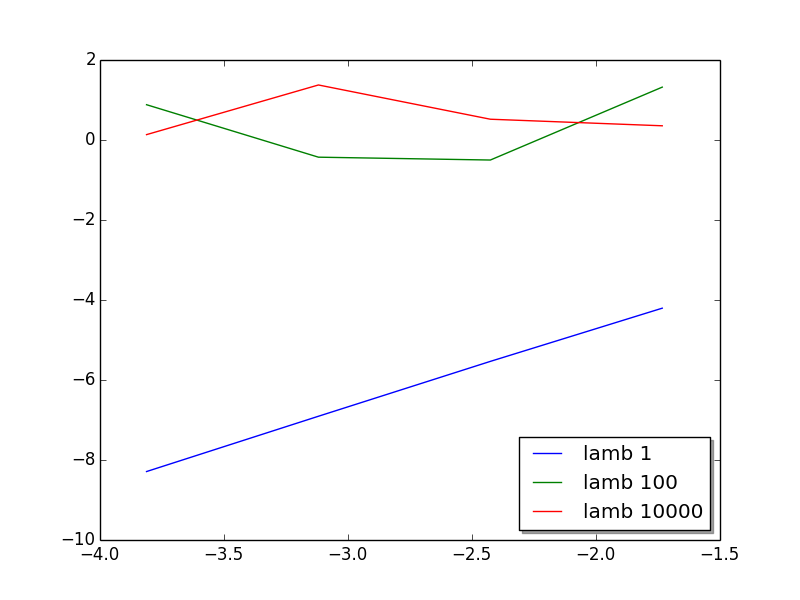
\includegraphics[scale=0.4]{log_plot_bad.png}   
    \caption{Log plot without trick}
    \label{fig:awesome_image}
    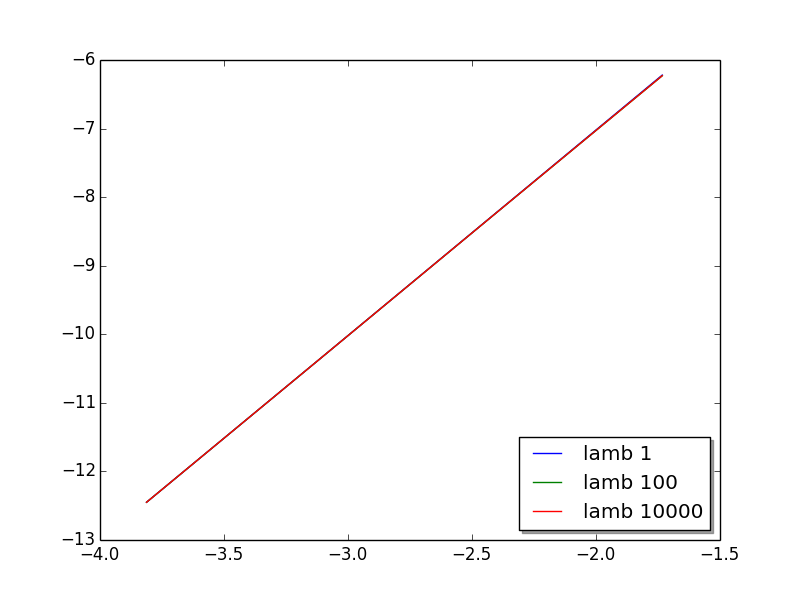
\includegraphics[scale=0.4]{log_plot_good.png}
    \caption{Log plot with trick}
    \label{fig:awesome_image}
\end{figure}
\newpage
\section*{Code}
\subsection*{7.6 Code}
\lstinputlisting[language=Python]{7_6.py}
\newpage
\subsection*{2 Code}
\lstinputlisting[language=Python]{ex_2.py}

















\end{document}